\subsection{MVC's architecture}
The MVC architecture holds:
\begin{itemize}
    \item \textbf{Models} - Holds the application state and simple operations to access/filter/manipulate
    that data. These operations are also called the Domain Logic.
    \item \textbf{Views} - the UI and pages build with the Flutter widgets. This layer may also contain the
    "view controllers" with handlers for local interactions.
    \item \textbf{Controller} - contains the Application Logic composed by the business operations that
    constitute the functionalities of the application. These operations can be organized in \textbf{Commands}
    invoked by the other layers, but mainly is result of UI interactions.
    \item \textbf{Services} - contain the operations in the outside world. Usually, they are invoked by
    Commands that can retrieve data and inject it on Models, or in the other direction.
\end{itemize}

\begin{figure}[h]
\centering
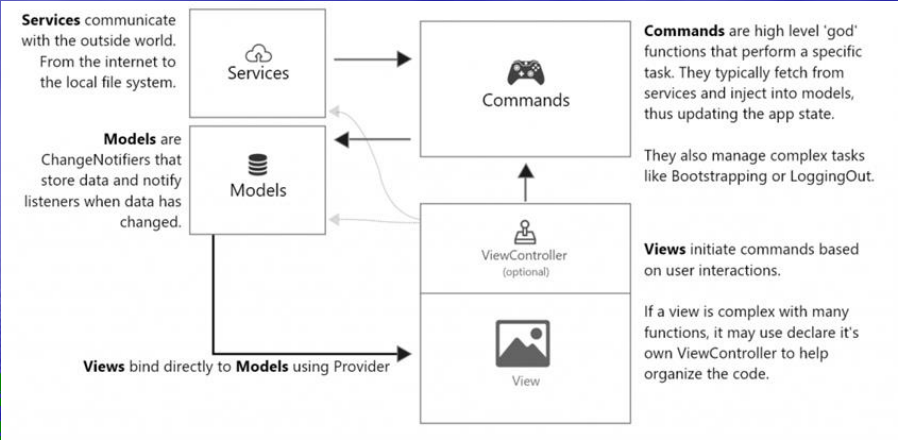
\includegraphics[width=0.8\linewidth]{figures/11_MVC_diagram.png}
\caption{MVC diagram}
\label{fig:mvc_diagram}
\end{figure}
\newpage
The implementation of this architecture requires access to the \texttt{Models} in every place in
the App. For doing that, a special widget is provided in an external package. It associates
\texttt{Models} and \texttt{Services} with the application context. The package is called \texttt{Provider}. 


\begin{figure}[h]
\centering
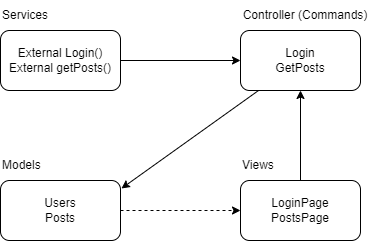
\includegraphics[width=0.6\linewidth]{figures/11_mvc_example_diagram.png}
\caption{MVC diagram example}
\label{fig:mvc_diagram_example}
\end{figure}

\subsection{Redux Architecture}
The Redux architecture specifies that all the application state is centralized in the
Store block (it can contain several Models). is a state management architecture library 
that successfully distributes data across widgets in a repetitive 
manner. It manages the state of an application through a unidirectional flow of data.

\begin{figure}[h]
\centering
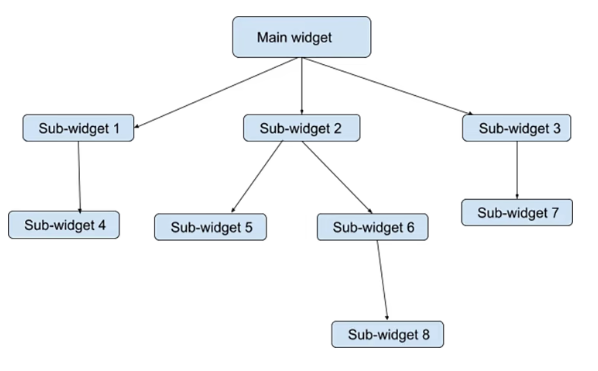
\includegraphics[width=0.4\linewidth]{figures/11_flow_data.png}
\caption{An unidirectional flow of data}
\label{fig:flow_data}
\end{figure}
In this example, data generated in the main widget is needed in sub-widget 8. 
Ordinarily, this data passes through sub-widget 2 to sub-widget 6 and then, finally, 
it reaches sub-widget 8. This is also the case for widgets that need data 
generated or saved in the state of any widget that's higher up in the hierarchy.

With Redux, \hl{you can structure your application so that the state is extracted in 
a centrally-located store. The data in this centralized store can be accessed 
by any widget that requires the data, without needing to pass through a chain of 
other widgets in the tree.}

Any widget that needs to add, modify, or retrieve the data in a state managed by the 
Redux store would have to request it with the appropriate arguments.

Likewise, for every change made to the state, the dependent widgets respond to the change 
either through the user interface or any other configured means.

\subsubsection{Why is it important?}
In a medium or large-scale application with many widgets, when a child widget needs data, 
it is common to manage the data from the main.dart file.

This data could be distributed through the constructors of widgets as arguments 
until the data gets to the recipient widget, 
\hl{this could lead to a long chain of data transfer through widgets that don't need this data.}

Not only can it be cumbersome and difficult to pass data through the constructors, 
\hl{it can also affect the performance of an application. This is because when you manage 
data from the main widget - or any root widget - the entire widget tree rebuilds 
whenever a change occurs in any of its child widgets}. You only want to run the 
build method in the widget that requires the changed data.

\subsubsection{How it works}
In Redux there's a \texttt{Store} which holds a \texttt{State} object that represents the 
\hl{state of the whole application}. Every application event (either from the user or external) 
is represented as an \texttt{Action} that gets dispatched to a \texttt{Reducer} function. 
This \hl{\texttt{Reducer} updates the \texttt{Store} with a new \texttt{State} depending on 
what \texttt{Action} it receives}.  
And whenever a new \texttt{State} is \hl{pushed (the state is immutable, thus it can't be 
modified, just replaced)}  through the \texttt{Store} the \texttt{View} is recreated to reflect 
the changes.

With Redux most components are decoupled, making UI changes very easy to make.
 In addition, the only business logic sits in the \texttt{Reducer} functions. 
 A \texttt{Reducer} is a function that takes an \texttt{Action} and the current application
  \texttt{State} and it returns a \hl{new} \texttt{State} object, therefore it is straightforward 
  to test because we can write a unit test that sets up an initial State and checks that 
  the \texttt{Reducer} returns the new and modified \texttt{State}.

\subsubsection{Middleware}
what happens when the application has to perform some asynchronous operation, such as 
loading data from an external API? This is why people came up with a new component
 known as the \texttt{Middleware}.

\texttt{Middleware} is a component that may process an \texttt{Action} before 
it reaches the \texttt{Reducer}. It receives the current application \texttt{State}
 and the \texttt{Action} that got dispatched, and it can run some code 
 (usually a side effect), such as communicating with a 3rd-party API or data source. 
 Finally, the \texttt{Middleware} may decide to dispatch the original \texttt{Action}, 
 to dispatch a different one, or to do nothing more. 
 
\subsubsection{Resume according to slides}
The \texttt{View} (flutter widget tree) generates \texttt{Actions} from user interactions, that specify
external requests and/or state modifications. The external requests are filtered out
by a \texttt{Middleware} block. The other \texttt{Actions} go to a \texttt{Reducer} function.

The \texttt{Reducer} function modifies the Store, according to the specified \texttt{Action}.
\texttt{Views} have access to the \texttt{Store}, and whenever this is modified it triggers a \texttt{View}
redrawing, taking into account the app state inside the \texttt{Store}.

\begin{figure}[h]
\centering
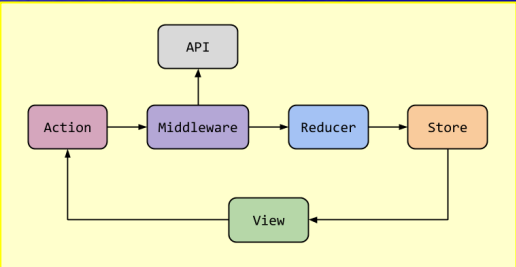
\includegraphics[width=0.8\linewidth]{figures/11_redux_diagram.png}
\caption{Redux architecture diagram}
\label{fig:redux_architecture_diagram}
\end{figure}
